\documentclass[../main.tex]{subfiles}

\begin{document}

\section{Threat model}
\label{section:problem:threat_model}

\par We will now look at the threat model of our system. To do so, we will use the STRIDE model developed by Microsoft instead of using an ad-hoc approach. STRIDE model allows us to be more structured and cover every security aspect that could be forgotten using an ad-hoc approach. We will define each aspect of STRIDE\footnote{Spoofing - Tampering - Repudiation - Information disclosure - Denial of service - Elevation of privilege} for each party acting in our system, which are: the \textbf{Cloud Provider}, the \textbf{auditor}, the \textbf{data owner} and the \textbf{authorised user}.\\

\par Firstly, we are going to look at the Cloud Provider. We consider him as an untrusted party to which no information can be disclosed and that is not trusted to hold any confidential data. We only consider the Cloud Provider to be honest, in the sense that he must correctly share data to users. With this in mind, the \textbf{Denial of service} aspect becomes irrelevant. As well as the Cloud \textbf{Spoofing} because an attacker must still correctly implement the sharing protocol.\\

\par Second, we consider all the other entities:
\par \textbf{Spoofing} any user is a mechanism whereby malicious actor impersonates our authorised user. This must be prevented as much as possible but as we will see later on, it is only feasible to a certain extent.
\par \textbf{Tampering} is relevant to all the parties. We must be able to detect when anyone is trying to change the content of a file to which he has not access\footnote{This also refers to users that are authorised to access a certain section of the filesystem and that wishes to tamper a section they don't have access to}.
\par \textbf{Repudiation} is only relevant for the authorised user. This must prevent the user from denying their action on the files. Related to this, we must enable forensic analysis indicating that a user tried to do something he is not allowed to (e.g: tamper with a file).
\par \textbf{Information disclosure} is obviously crucial is our scenario, however become irrelevant with authorised user. There is no way to build a system that prevent authorised users from making the information public.
\par \textbf{Denial of service} means that the user voluntary stops to download or upload information to the Cloud storage. This is considered irrelevant here because we consider every user to be honest. As with the Cloud Provider this means that they follow the protocol, which means that they upload or download information as soon as they can.
\par \textbf{Elevation of privilege} for all the users means that they can't change their role. Concerning the authorised user this also means that he can't, in any way, change any entitlements.\\

\par A synthesis of this threat model along with a reminder of the role of each party can be found in the following Figure:
\begin{figure}[h]
    \centering
    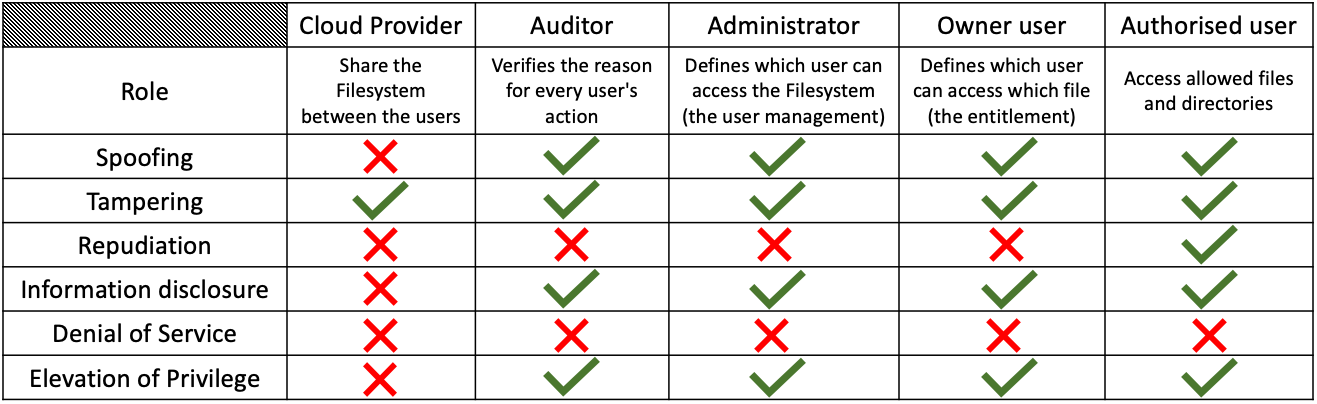
\includegraphics[width=0.75\textwidth]{images/problem/threat_model}
    
    \caption{Threat model}
    \label{figure:problem:threat_model}
\end{figure}


\end{document} 